\documentclass[fontsize=9pt,twocolumns,enabledeprecatedfontcommands]{scrartcl}
\usepackage[a4paper,textwidth=0.85\paperwidth,textheight=0.80\paperheight]{geometry}
%\usepackage[a4paper]{geometry}
\setlength{\columnsep}{0.03\paperwidth}

\usepackage[utf8]{inputenc}
\usepackage[english]{babel}
\usepackage[T1]{fontenc}
\usepackage{amsmath}
\usepackage{amsfonts}
\usepackage{amssymb}
\usepackage{epigraph}
\usepackage{paralist}
\usepackage{mathtools}%for smash operator

\usepackage{indentfirst} %adds indentation after sectioning

\usepackage{graphicx}
\usepackage{amsthm}
\usepackage{stmaryrd}  %pour Mapsto

\usepackage[bf,format=plain]{caption}
\usepackage{subcaption}
\usepackage{dblfloatfix}

\usepackage{url}
\usepackage{hyperref}
\usepackage{csquotes}

\usepackage[usenames,dvipsnames]{color}

\usepackage{algpseudocode}


\renewcommand\thesubfigure{\arabic{figure}} %subfigure have same counter as figures

\newcommand{\HRule}{\rule{0.9\linewidth}{0.05em}}

\addtokomafont{sectioning}{\rmfamily}
%\addtokomafont{part}{\huge}

\def\labelitemi{\textbf{--}}
\newenvironment{itemize'}
{ %\vspace{-0.75\topsep}
  \begin{itemize}
    \vspace{-\topsep}
    \setlength{\itemsep}{0pt}
    \setlength{\parskip}{0pt}
    \setlength{\parsep}{0pt}     }
{ \end{itemize} \vspace{-0.75\topsep}                 } 


\begin{document}
%\newgeometry{textheight=0.80\paperheight,textwidth=0.7\paperwidth}
%\begin{figure*}[h!]
\twocolumn[{
\noindent
\sffamily
\begin{center}
{\Large { Centre de Recherches Interdisciplinaires |  M1 AIV}}
%\\[1em]

\HRule

\vspace{1em}
{\Huge Solving optimization problems with search heuristics }\\[0.7em]

{\Huge Project report
}

\HRule
\\[2em]

\LARGE
\begin{tabular}{c}
	Arthur Carcano\\
\end{tabular}
\vspace{1em}
%\vfill
\end{center}}]


\newcommand{\wip}[1]{\textcolor{Purple}{WIPWIPWIPWIP #1 WIPWIPWIPWIP}}

\begin{abstract}
	We hereby present our solution to the traveling thief problem. Using a two phase algorithm inspired by \cite{Polyakovkiy}, we manage to reach solutions of about $16k$ on the \texttt{a280\_n279\_bounded-strongly-corr\_01.ttp} instance.
\end{abstract}

\section{Our algorithm}
Following the idea of Polyakovsiy \textit{et al.} \cite{Polyakovskiy} our algorithm runs in two phases. First a run for the travellign salesman problem is generated. Second, using this run, the algorithm plans which objects are to be picked up so as to maximize the total profit of our thief.

It is noteworthy that, whereas our algorithm for the first phase is kind of intricate, the one used for the second phase is merely a classical simulated annealing.

\subsection{The TSP algorithm}
To solve the TSP problem, we first build a greedy solution on which we run an exhaustive 2-opt, and which we then improve with different heuristics: basic node permutation, \textit{2-opt} and an permutation we call \textit{stitching} which is actually a specialization of \textit{3-opt}. A possible output is given figure \ref{tsp_sol}.

\begin{figure}[hp]
	\centering
	\includegraphics[width=0.9\linewidth]{tsp}
	\label{tsp_sol}
	\caption{A possible tour, as foudn by our algorithm.}
\end{figure}


Both node inversion and stitching are accepting with a probability depending on a temperature $T$ that is exponentially decreasing.\\

We introduce the following notation, for any $x \in \mathcal{R}_+$ we define $\overline{x} = \max(1,x)$.

\subsubsection{Node inversion}:
This operation simply picks two nodes uniformly at random, compute $\Delta$ the difference of length of the tour if this two nodes are permuted and actually does this permutation with probability $\overline{e^{\frac{-\Delta}{T}}}$.

\subsubsection{Stitching}:
\begin{figure}[htbp]
	\centering
	
	\begin{subfigure}{0.4\textwidth}
		
		\centering
		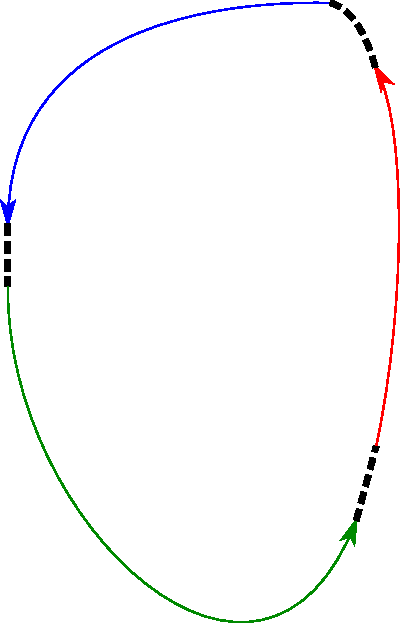
\includegraphics[angle=90,width=\linewidth,height=0.15\textheight]{stitch1}
		\caption{Before stitching}
		\label{stitch1}
		
	\end{subfigure}
	\vspace{2em}
	\begin{subfigure}{0.4\textwidth}
		
		\centering
		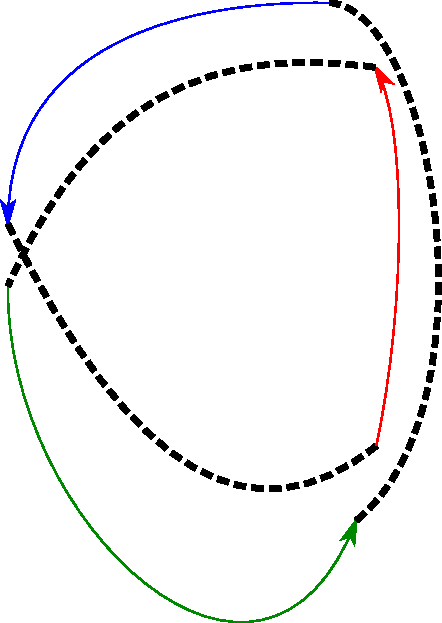
\includegraphics[angle=90,width=\linewidth,height=0.15\textheight]{stitch2}
		\caption{After stitching}
		\label{stitch2}
		
	\end{subfigure}
	\captionsetup{format=plain}
	\caption{Illustration of the stitching operation}
	\label{stitch_fig}
\end{figure}

As illustrated in figure \ref{stitch_fig}, the stitching operation consist in "inserting a part of the tour between two nodes". As with the nodes inversion, this is only done with probability $\overline{e^{\frac{-\Delta}{T}}}$.

\subsubsection{2-opt}
Two opt is plentifully described in literature. We simply implement it with a selection of the points at random. 

\subsection{Knapsack}
Once the tour is generated, we still have to choose wich items to pick up. To this end, we simply use the RLS algorithm described in \cite{Polyakovskiy}.

\subsection{Number of iterations}
Because we need to run two optimizing heuristics one after the other, we must give a way to the algorithm to decide whether or not it has reached a good solution for the TSP. Because the keystone of our algorithm is the random selection of two (for 2-opt and node inversion) or three (for stitching) nodes, and because the expected run time of a coupon collector on $n^2$ entries is about $2n^2\ln(n)$, we say that our algorithm is done once there have been $4n^2\ln(n)$ iteration without improving the score, which gives a probability $1/n$ of having missed some couple of points.

As is often the case when doing simulated annealing, we do several run of the "optimization with decreasing temperature" part. This gives the overall algorithm in figure \ref{algo}

\begin{figure}
\begin{algorithmic}
	\State Generate greedy TSP
	\State do one exhaustive 2-opt
\For {$i \in 0..10$}
	\State temp = 1
	\While{One of the last $4n^2\ln(n)$ iterations has improved the score}
	\State do 4 RLS for inversion
	\State do 1 RLS for 2-opt
	\State do 1 RLS for stitching
	\State temp $/=$ 0.9999
	\EndWhile
	\EndFor
\For {$i \in 0..10$}
\State temp = 100	
	\While{One of the last $2n\ln(n)$ iterations has improved the score}
	\State do 1 RLS
	\State temp $/=$ 0.9999
	\EndWhile
	\EndFor

\end{algorithmic}
\label{algo}
\caption{Our algorithm}
\end{figure} 

\section{Results}




\bibliographystyle{siam}
\bibliography{biblio}

\end{document}



%\begin{abstract}
